% Standalone TikZ figures for MOAI-LoRA paper
% Compile individually with: pdflatex -shell-escape figures.tex

\documentclass[tikz,border=10pt]{standalone}
\usepackage{tikz}
\usetikzlibrary{shapes,arrows,positioning,fit,backgrounds,calc,matrix}
\usepackage{amsmath}

% Define colors
\definecolor{ckksblue}{RGB}{66,133,244}
\definecolor{tfhepurple}{RGB}{156,39,176}
\definecolor{loragreen}{RGB}{52,168,83}
\definecolor{privacyred}{RGB}{234,67,53}
\definecolor{lightgray}{RGB}{245,245,245}

\begin{document}

%==============================================================================
% Figure 1: MOAI-LoRA System Architecture
%==============================================================================
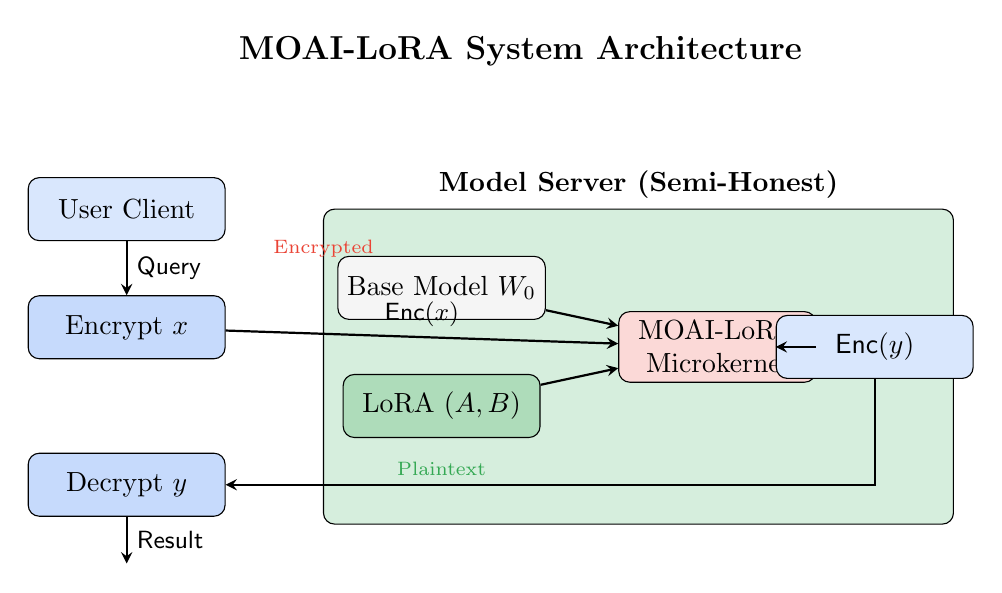
\begin{tikzpicture}[
    box/.style={draw, rounded corners, minimum width=2.5cm, minimum height=0.8cm, align=center},
    arrow/.style={->, thick, >=stealth},
    label/.style={font=\small\sffamily}
]

% Title
\node[font=\large\bfseries] at (5, 6) {MOAI-LoRA System Architecture};

% User side
\node[box, fill=ckksblue!20] (user) at (0, 4) {User Client};
\node[box, fill=ckksblue!30] (encrypt) at (0, 2.5) {Encrypt $x$};
\node[box, fill=ckksblue!30] (decrypt) at (0, 0.5) {Decrypt $y$};

% Server side
\node[box, fill=loragreen!20, minimum width=8cm, minimum height=4cm] (server) at (6.5, 2) {};
\node[font=\bfseries, above] at (server.north) {Model Server (Semi-Honest)};

% Inside server
\node[box, fill=lightgray] (base) at (4, 3) {Base Model $W_0$};
\node[box, fill=loragreen!40] (lora) at (4, 1.5) {LoRA $(A, B)$};
\node[box, fill=privacyred!20] (moai) at (7.5, 2.25) {MOAI-LoRA\\Microkernel};
\node[box, fill=ckksblue!20] (output) at (9.5, 2.25) {$\mathsf{Enc}(y)$};

% Arrows
\draw[arrow] (user) -- node[right, label] {Query} (encrypt);
\draw[arrow] (encrypt) -- node[above, label] {$\mathsf{Enc}(x)$} (moai);
\draw[arrow] (base) -- (moai);
\draw[arrow] (lora) -- (moai);
\draw[arrow] (moai) -- (output);
\draw[arrow] (output) |- (decrypt);
\draw[arrow] (decrypt) -- node[right, label] {Result} ($(decrypt)-(0,1)$);

% Annotations
\node[font=\scriptsize, text=privacyred] at (2.5, 3.5) {Encrypted};
\node[font=\scriptsize, text=loragreen] at (4, 0.7) {Plaintext};

\end{tikzpicture}

%==============================================================================
% Figure 2: Column-Packed Matrix Multiplication
%==============================================================================
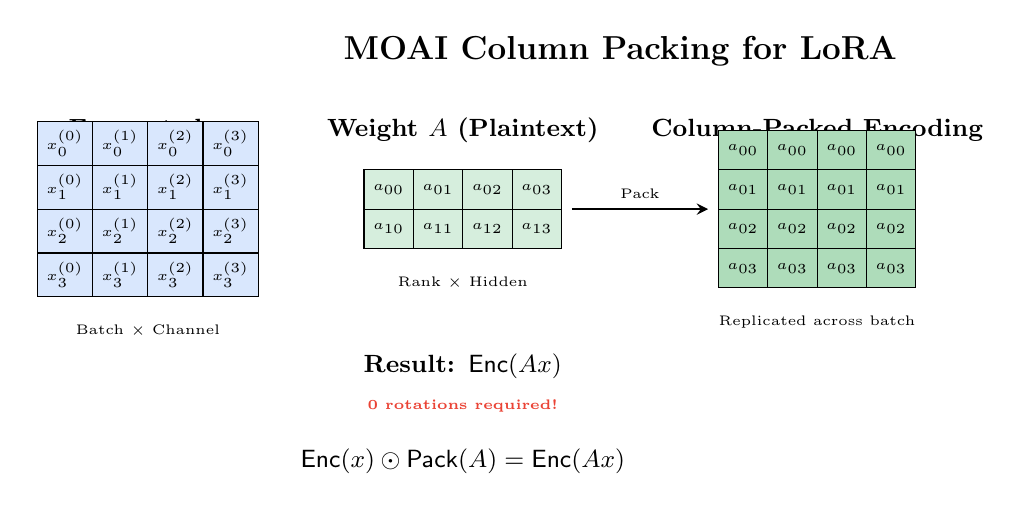
\begin{tikzpicture}[
    slot/.style={draw, minimum width=0.5cm, minimum height=0.5cm, font=\tiny},
    arrow/.style={->, thick, >=stealth}
]

% Title
\node[font=\large\bfseries] at (6, 5.5) {MOAI Column Packing for LoRA};

% Input ciphertext
\node[font=\small\bfseries] at (0, 4.5) {Encrypted $x$};
\matrix[matrix of nodes, nodes={slot, fill=ckksblue!20}, row sep=-\pgflinewidth, column sep=-\pgflinewidth] (ct) at (0, 3.5) {
    $x_0^{(0)}$ & $x_0^{(1)}$ & $x_0^{(2)}$ & $x_0^{(3)}$ \\
    $x_1^{(0)}$ & $x_1^{(1)}$ & $x_1^{(2)}$ & $x_1^{(3)}$ \\
    $x_2^{(0)}$ & $x_2^{(1)}$ & $x_2^{(2)}$ & $x_2^{(3)}$ \\
    $x_3^{(0)}$ & $x_3^{(1)}$ & $x_3^{(2)}$ & $x_3^{(3)}$ \\
};
\node[font=\tiny, below=0.1cm of ct] {Batch $\times$ Channel};

% Weight matrix (plaintext)
\node[font=\small\bfseries] at (4, 4.5) {Weight $A$ (Plaintext)};
\matrix[matrix of nodes, nodes={slot, fill=loragreen!20}, row sep=-\pgflinewidth, column sep=-\pgflinewidth] (wt) at (4, 3.5) {
    $a_{00}$ & $a_{01}$ & $a_{02}$ & $a_{03}$ \\
    $a_{10}$ & $a_{11}$ & $a_{12}$ & $a_{13}$ \\
};
\node[font=\tiny, below=0.1cm of wt] {Rank $\times$ Hidden};

% Column packed encoding
\node[font=\small\bfseries] at (8.5, 4.5) {Column-Packed Encoding};
\matrix[matrix of nodes, nodes={slot, fill=loragreen!40}, row sep=-\pgflinewidth, column sep=-\pgflinewidth] (packed) at (8.5, 3.5) {
    $a_{00}$ & $a_{00}$ & $a_{00}$ & $a_{00}$ \\
    $a_{01}$ & $a_{01}$ & $a_{01}$ & $a_{01}$ \\
    $a_{02}$ & $a_{02}$ & $a_{02}$ & $a_{02}$ \\
    $a_{03}$ & $a_{03}$ & $a_{03}$ & $a_{03}$ \\
};
\node[font=\tiny, below=0.1cm of packed] {Replicated across batch};

% Arrows
\draw[arrow] (wt) -- node[above, font=\tiny] {Pack} (packed);

% Result
\node[font=\small\bfseries] at (4, 1.5) {Result: $\mathsf{Enc}(Ax)$};
\node[font=\tiny, text=privacyred] at (4, 1) {\textbf{0 rotations required!}};

% Equation
\node[font=\small] at (4, 0.3) {$\mathsf{Enc}(x) \odot \mathsf{Pack}(A) = \mathsf{Enc}(Ax)$};

\end{tikzpicture}

%==============================================================================
% Figure 3: Rotation Comparison
%==============================================================================
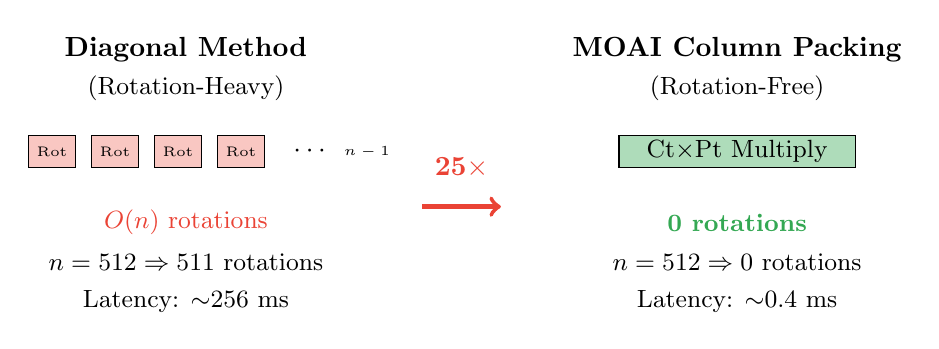
\begin{tikzpicture}
    \begin{scope}[shift={(0,0)}]
        % Naive approach
        \node[font=\bfseries] at (2, 4) {Diagonal Method};
        \node[font=\small] at (2, 3.5) {(Rotation-Heavy)};

        \foreach \i in {0,1,2,3} {
            \draw[fill=privacyred!30] (\i*0.8, 2.5) rectangle (\i*0.8+0.6, 2.9);
            \node[font=\tiny] at (\i*0.8+0.3, 2.7) {Rot};
        }
        \node at (3.6, 2.7) {$\cdots$};
        \node[font=\tiny] at (4.3, 2.7) {$n-1$};

        \node[font=\small, text=privacyred] at (2, 1.8) {$O(n)$ rotations};
        \node[font=\small] at (2, 1.3) {$n=512 \Rightarrow 511$ rotations};
        \node[font=\small] at (2, 0.8) {Latency: $\sim$256 ms};
    \end{scope}

    \begin{scope}[shift={(7,0)}]
        % MOAI approach
        \node[font=\bfseries] at (2, 4) {MOAI Column Packing};
        \node[font=\small] at (2, 3.5) {(Rotation-Free)};

        \draw[fill=loragreen!40] (0.5, 2.5) rectangle (3.5, 2.9);
        \node[font=\small] at (2, 2.7) {Ct$\times$Pt Multiply};

        \node[font=\small, text=loragreen] at (2, 1.8) {\textbf{0 rotations}};
        \node[font=\small] at (2, 1.3) {$n=512 \Rightarrow 0$ rotations};
        \node[font=\small] at (2, 0.8) {Latency: $\sim$0.4 ms};
    \end{scope}

    % Speedup arrow
    \draw[->, ultra thick, privacyred] (5, 2) -- (6, 2);
    \node[font=\bfseries, text=privacyred] at (5.5, 2.5) {25$\times$};

\end{tikzpicture}

%==============================================================================
% Figure 4: Hybrid CKKS-TFHE Pipeline
%==============================================================================
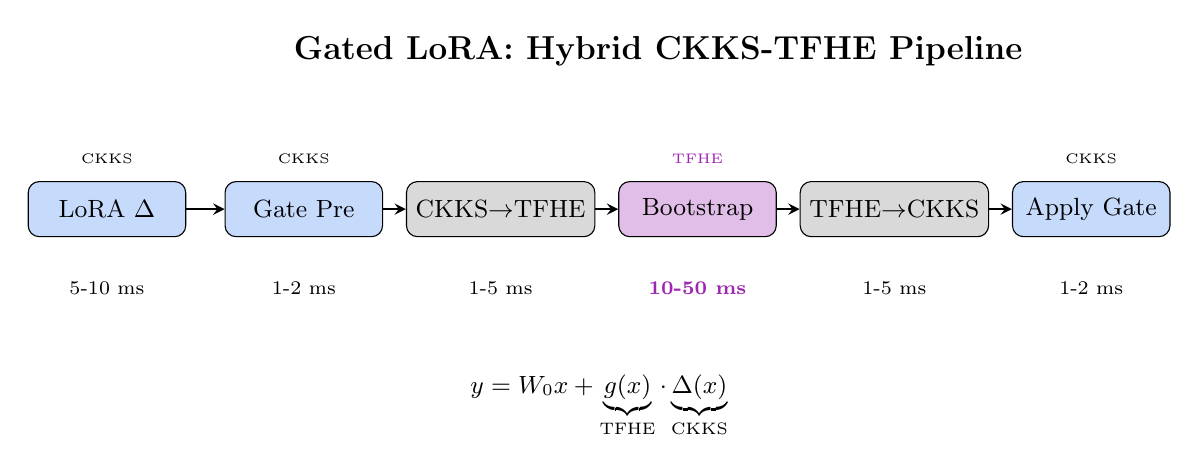
\begin{tikzpicture}[
    phase/.style={draw, rounded corners, minimum width=2cm, minimum height=0.7cm, font=\small},
    arrow/.style={->, thick, >=stealth}
]

% Title
\node[font=\large\bfseries] at (7, 5) {Gated LoRA: Hybrid CKKS-TFHE Pipeline};

% CKKS phases
\node[phase, fill=ckksblue!30] (p1) at (0, 3) {LoRA $\Delta$};
\node[phase, fill=ckksblue!30] (p2) at (2.5, 3) {Gate Pre};

% Bridge
\node[phase, fill=gray!30] (bridge1) at (5, 3) {CKKS$\to$TFHE};

% TFHE phase
\node[phase, fill=tfhepurple!30] (p3) at (7.5, 3) {Bootstrap};

% Bridge back
\node[phase, fill=gray!30] (bridge2) at (10, 3) {TFHE$\to$CKKS};

% Final CKKS
\node[phase, fill=ckksblue!30] (p4) at (12.5, 3) {Apply Gate};

% Arrows
\draw[arrow] (p1) -- (p2);
\draw[arrow] (p2) -- (bridge1);
\draw[arrow] (bridge1) -- (p3);
\draw[arrow] (p3) -- (bridge2);
\draw[arrow] (bridge2) -- (p4);

% Labels
\node[font=\tiny, above=0.1cm of p1] {CKKS};
\node[font=\tiny, above=0.1cm of p2] {CKKS};
\node[font=\tiny, above=0.1cm of p3, text=tfhepurple] {TFHE};
\node[font=\tiny, above=0.1cm of p4] {CKKS};

% Timing
\node[font=\scriptsize] at (0, 2) {5-10 ms};
\node[font=\scriptsize] at (2.5, 2) {1-2 ms};
\node[font=\scriptsize] at (5, 2) {1-5 ms};
\node[font=\scriptsize, text=tfhepurple] at (7.5, 2) {\textbf{10-50 ms}};
\node[font=\scriptsize] at (10, 2) {1-5 ms};
\node[font=\scriptsize] at (12.5, 2) {1-2 ms};

% Equation
\node[font=\small] at (6.25, 0.5) {$y = W_0 x + \underbrace{g(x)}_{\text{TFHE}} \cdot \underbrace{\Delta(x)}_{\text{CKKS}}$};

\end{tikzpicture}

%==============================================================================
% Figure 5: Throughput Comparison Bar Chart
%==============================================================================
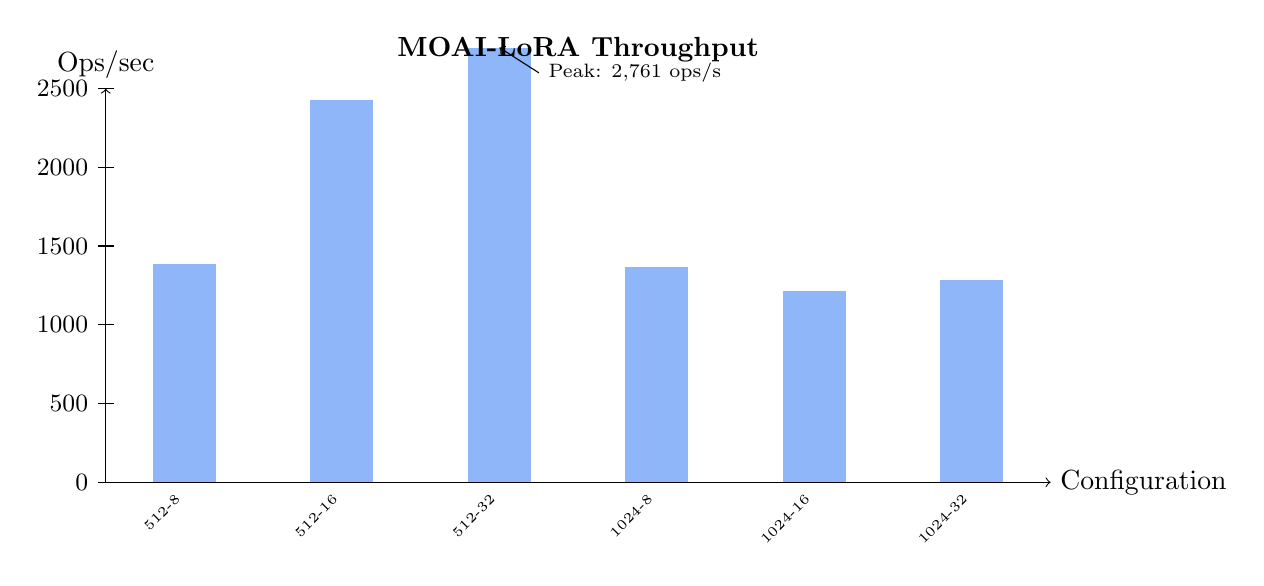
\begin{tikzpicture}
    % Axes
    \draw[->] (0, 0) -- (12, 0) node[right] {Configuration};
    \draw[->] (0, 0) -- (0, 5) node[above] {Ops/sec};

    % Y-axis labels
    \foreach \y/\label in {0/0, 1/500, 2/1000, 3/1500, 4/2000, 5/2500} {
        \draw (-0.1, \y) -- (0.1, \y);
        \node[left] at (-0.1, \y) {\small \label};
    }

    % Bars
    \foreach \x/\h/\label in {1/2.77/512-8, 3/4.86/512-16, 5/5.52/512-32, 7/2.74/1024-8, 9/2.43/1024-16, 11/2.57/1024-32} {
        \fill[ckksblue!60] (\x-0.4, 0) rectangle (\x+0.4, \h);
        \node[below, font=\tiny, rotate=45, anchor=east] at (\x, -0.1) {\label};
    }

    % Title
    \node[font=\bfseries] at (6, 5.5) {MOAI-LoRA Throughput};

    % Peak annotation
    \draw[->] (5.5, 5.2) -- (5, 5.52);
    \node[font=\scriptsize, right] at (5.5, 5.2) {Peak: 2,761 ops/s};

\end{tikzpicture}

%==============================================================================
% Figure 6: Latency Comparison
%==============================================================================
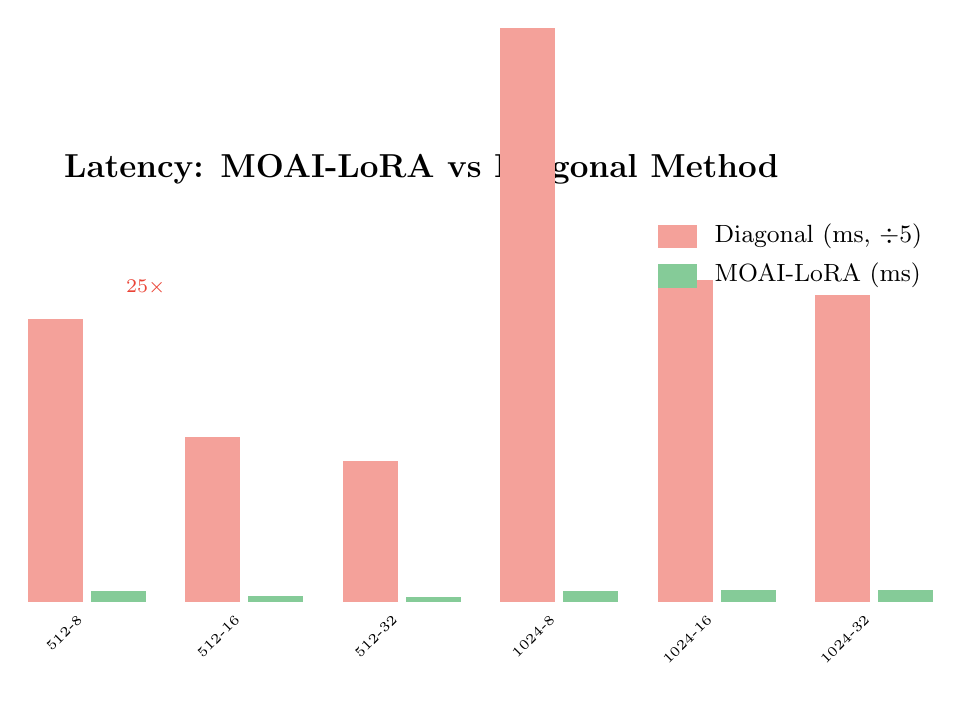
\begin{tikzpicture}
    % Title
    \node[font=\large\bfseries] at (5, 5.5) {Latency: MOAI-LoRA vs Diagonal Method};

    % Bars - Diagonal (log scale approximation)
    \foreach \x/\d/\m/\label in {0/3.6/0.14/512-8, 2/2.1/0.08/512-16, 4/1.8/0.07/512-32, 6/7.3/0.15/1024-8, 8/4.1/0.16/1024-16, 10/3.9/0.16/1024-32} {
        % Diagonal bar (scaled down for visualization)
        \fill[privacyred!50] (\x, 0) rectangle (\x+0.7, \d);
        % MOAI bar
        \fill[loragreen!60] (\x+0.8, 0) rectangle (\x+1.5, \m);
        % Label
        \node[below, font=\tiny, rotate=45, anchor=east] at (\x+0.75, -0.1) {\label};
    }

    % Legend
    \fill[privacyred!50] (8, 4.5) rectangle (8.5, 4.8);
    \node[right, font=\small] at (8.6, 4.65) {Diagonal (ms, $\div$5)};
    \fill[loragreen!60] (8, 4) rectangle (8.5, 4.3);
    \node[right, font=\small] at (8.6, 4.15) {MOAI-LoRA (ms)};

    % Speedup annotations
    \node[font=\scriptsize, text=privacyred] at (1.5, 4) {25$\times$};

\end{tikzpicture}

\end{document}
